\subsection{Integration Reverse Proxy}
\label{sec:integration-reverse-proxy}

Mit dem \nameref{sec:proteciton-reverse-proxy} können Web- und Applikationsserver bereits vom eigentlichen Berührungspunkt mit dem Internet separiert werden. Durch die Erweiterung des Konzepts zum \emph{Integration Reverse Proxy} kann das ganze System nun auch unabhängig von physischer und logischer Struktur bereitgestellt und angesprochen werden.

\subsection*{Kontext}
Ein System, bestehend aus mehreren Web- und Applikationsservern soll transparent angesprochen werden können.

\subsection*{Problem}
Verschiedene Web- und Applikationsserver bilden ein Gesamtsystem. Im einfachsten Fall ist jeder Server über ein eindeutige URL erreichbar (bspw. ``shop.business.com'', ``info.business.com'' usw.). Auf diese Weise wird die interne Systemstruktur unweigerlich nach Aussen sichtbar gemacht. Zudem kann der Ausfall einzelner Komponenten zu grösseren Problemen führen, da bspw. ein Load Balancing nicht ohne weiteres machbar ist.

Wie kann ein solcher Verbund von Servern für den Aussenstehenden transparent verfügbar gemacht werden, wenn folgende Faktoren eine Rolle spielen?

\begin{itemize}
	\item Die Implementation auf einem einzigen physischen Server ist keine Option (Fehlertoleranz etc.)
	\item Die grundlegende Netzwerkstruktur (Hosts etc.) soll nicht nach Aussen getragen werden
	\item Einzelne Systemkomponenten sollen problemlos untereinander kommunizieren können (keine Hardlinks mit IP's o.Ä.)
	\item Ergänzung, Austausch und bis zu einem gewissen Mass Entfernung von Komponenten soll andere Komponenten nicht beeinflussen
	\item Load Balancing auf mehrere Komponenten soll möglich sein
	\item Optimalerweise muss lediglich ein einziges SSL Zertifikat angeschafft werden (Kosten)
\end{itemize}

\newpage
\subsection*{Lösung}
Analog zum \nameref{sec:proteciton-reverse-proxy} wird ein \emph{Integration Reverse Proxy} ins System integriert.

\begin{figure}[H]
	\centering
	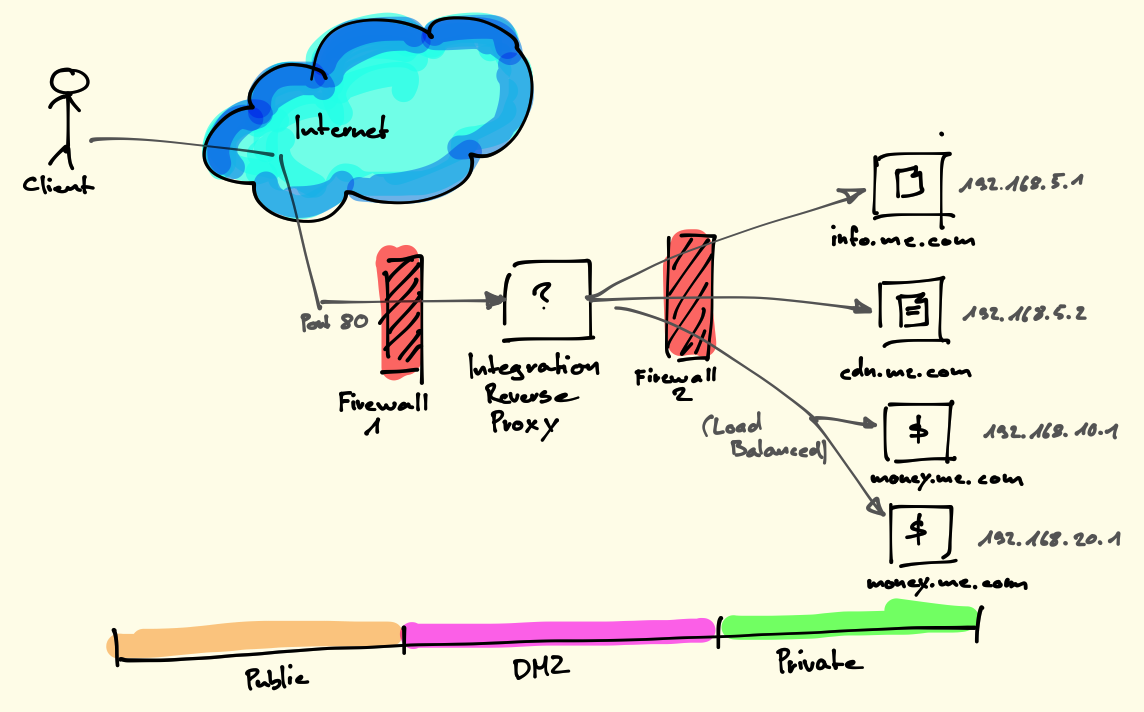
\includegraphics[width=12cm]{content/security/secure-internet-applications/images/integration-reverse-proxy.png}
	\caption{Strutkureller Aufbau Integration Reverse Proxy}
\end{figure}

Neben der einfachen Überprüfung und Weiterleitung von Requests wird nun selektiv entschieden, an welchen Server im eigenen Netz der jeweilige Request weitergeleitet werden soll.


\subsection*{Vorteile}
\begin{itemize}
	\item Lediglich ein einziger Server/Host ist von Aussen erreichbar
	\item Die interne Netzwerkstruktur wird nicht preisgegeben
	\item Einzelne Komponenten können problemlos ausgetauscht werden oder auch nur temporär durch andere ersetzt werden: Alles eine Frage der Konfiguration des \emph{Integration Reverse Proxy}
	\item Ein zentralisiertes Logging über verschiedene Systemkomponenten wird ermöglicht
	\item Nur ein einziges, teures SSL Zertifikat. Statt mehrere. Yay! ;)
\end{itemize}

\subsection*{Nachteile}
Neben den vom \nameref{sec:proteciton-reverse-proxy} bekannten Nachteile kommen folgende hinzu:

\begin{itemize}
	\item Die max. Anzahl von Netzwerk-Verbindungen ist begrenzt! Diese Limitierung kann umgangen werden, indem bspw. bereits beim DNS-Server ein Load Balancing umgesetzt wird, welches nicht immer auf den selben \emph{Integration Reverse Proxy} verweist.
	\item Testing-Aufwand steigt, da höhere Komplexität im Gesamtsystem
\end{itemize}

\subsection*{Reallife Beispiele}
\begin{itemize}
	\item Viele Ruby- oder Node.JS-Applikationen (Liste nicht abschliessend ;) ) verfügen über einen eigenen Webserver. Möchte man diese über einen bestehenden Webserver (z.B. nginx oder Apache) verfügbar machen, kommt ein entsprechendes \emph{Reverse Proxy}-Modul zum Einsatz.
	Zwar laufen diese Applikationen im einfachsten Falle dann auf dem selben Host und ohne zusätzlich dazwischengeschaltete Firewall, die Technik an sich bleibt jedoch die gleiche wie beim voll ausgebauten Pattern.
\end{itemize}